% !TEX TS-program = XeLaTeX
% !TEX spellcheck = en-US
\documentclass[aspectratio=169]{beamer}
\usepackage{tikz}
\usetikzlibrary{positioning}
\newcommand{\high}[1]{{\color{red}#1}}

\usetheme{example}

\title{Lecture 8:\\ Backpropagation and Gradient Descent}
\institute{GRA4160: Predictive modelling with machine learning}
\date{February 27st 2025}
\author{Vegard H\o ghaug Larsen}

\begin{document}

\maketitle

\frame{
    \frametitle{Plan for today:}
    \begin{itemize}
        \item \textbf{Topic:} \textit{Backpropagation and Gradient Descent} - understanding how neural networks learn  
        \item \textbf{Key Concepts:} Gradient descent variants, computational graphs, the chain rule, backpropagation algorithm  
        \item \textbf{Approach:} Start from first principles, then live-code a simple automatic differentiation engine 
        \item \textbf{Goal:} Build intuition on how gradients are computed and used to train models
    \end{itemize}
    Two examples:
    \begin{itemize}
        \item ADALINE for binary classification
        \item Logistic regression
    \end{itemize}
}

\frame{
    \frametitle{What is Gradient Descent?}
    \begin{itemize}
        \item An optimization algorithm to \textbf{minimize a loss function} by iteratively moving in the direction of \textbf{steepest descent} (negative gradient).  
        \item \textbf{Update rule:} For a parameter $w$, 
        \[w \leftarrow w - \eta \,\nabla_w L,\] 
        where $\eta$ is the learning rate (step size).  
        \item \textbf{Objective:} find parameters that minimize the loss (error) on training data, by continuously updating weights opposite to the gradient.
    \end{itemize}
}

\frame{
    \frametitle{What is the gradient?}
    \begin{itemize}
        \item By gradient we mean the \textbf{partial derivatives} of the loss with respect to the parameters.
        \item \textbf{Gradient:} with two parameters $w_1$ and $w_2$, the gradient of the loss with respect to a parameter $w_i$ is given by 
        \[\nabla_{w_i} L = \frac{\partial L}{\partial w_i}.\]
        \item \textbf{Gradient vector:} the gradient vector is given by 
        \[\nabla_w L = \left(\frac{\partial L}{\partial w_1}, \frac{\partial L}{\partial w_2}\right).\]
        \item The gradient vector points in the direction of the steepest ascent of the loss function.
    \end{itemize}
}

\frame{
    \frametitle{Gradient Descent Variants}
    \begin{itemize}
        \item \textbf{Batch Gradient Descent:} Compute gradient on the entire dataset before each update - stable but can be very slow for large data.
        \item \textbf{Stochastic Gradient Descent (SGD):} Compute gradient on a single example at a time - much faster updates but noisier (updates may fluctuate).
        \item \textbf{Mini-Batch Gradient Descent:} Compute gradient on a small batch of examples (e.g. 32 or 64) - a compromise that offers faster convergence than full-batch and more stability than pure SGD.
        \item In practice, mini-batches are most common (e.g. 32 samples per update) to leverage vectorized computation and achieve good convergence.
    \end{itemize}
}

\frame{
    \frametitle{Computational Graphs}
    A computational graph is a directed graph representing the flow of data through a sequence of operations. 
    \begin{itemize}
        \item Nodes are operations or variables; edges show dependencies.
        \item Example: The expression 
        \[L(w_1, w_2) = ((w_1 - 1)^2 + (w_2 - 5)^2) \times 0.5\] 
        can be represented as a graph of simpler operations (subtraction, square, addition, multiply).
    \end{itemize}
}

\frame{
    \frametitle{Computational Graphs: a loss function}
    \begin{center}
        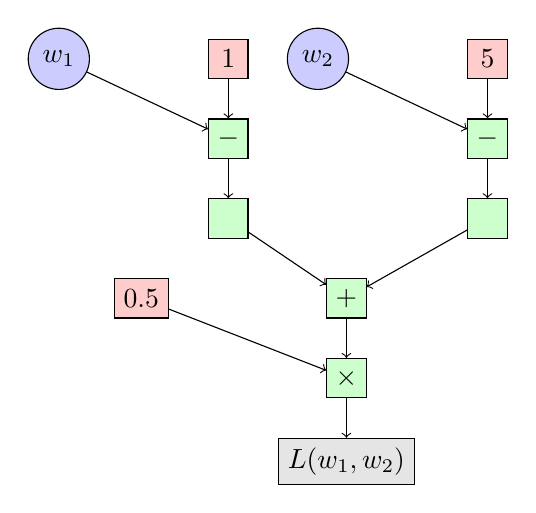
\begin{tikzpicture}[node distance=0.5cm, auto,
            input/.style={draw, circle, fill=blue!20, minimum size=0.5cm},
            const/.style={draw, rectangle, fill=red!20, minimum size=0.5cm},
            op/.style={draw, shape=rectangle, fill=green!20, inner sep=2pt, minimum width=0.5cm, minimum height=0.5cm},
            output/.style={draw, rectangle, fill=gray!20, minimum size=0.5cm}]
        
            % Layer 1: Inputs & constants for subtraction
            \node[input] (w1) {$w_1$};
            \node[input, right=2.5cm of w1] (w2) {$w_2$};
            \node[const, right=of w1, xshift=1.0cm] (c1) {1};
            \node[const, right=of w2, xshift=1.0cm] (c2) {5};
        
            % Layer 2: Subtraction operations
            \node[op, below=of c1] (sub1) {$-$};
            \node[op, below=of c2] (sub2) {$-$};
        
            % Layer 3: Squaring operations
            \node[op, below=of sub1] (sq1) {$\square$};
            \node[op, below=of sub2] (sq2) {$\square$};
        
            % Layer 4: Addition of squares
            \node[op, below=of sq1, xshift=1.5cm] (add) {$+$};
        
            % Layer 5: Constant for multiplication
            \node[const, left=of add, xshift=-1.5cm] (half) {0.5};
        
            % Layer 6: Multiplication to produce loss
            \node[op, below=of add] (mul) {$\times$};
        
            % Layer 7: Loss output
            \node[output, below=of mul] (loss) {$L(w_1, w_2)$};
        
            % Draw arrows from inputs to subtraction nodes
            \draw[->] (w1) -- (sub1);
            \draw[->] (c1) -- (sub1);
            \draw[->] (w2) -- (sub2);
            \draw[->] (c2) -- (sub2);
        
            % From subtraction to squaring
            \draw[->] (sub1) -- (sq1);
            \draw[->] (sub2) -- (sq2);
        
            % From squaring to addition
            \draw[->] (sq1) -- (add);
            \draw[->] (sq2) -- (add);
        
            % From multiplication constant and addition to multiplication node
            \draw[->] (half) -- (mul);
            \draw[->] (add) -- (mul);
        
            % Finally, multiplication to loss
            \draw[->] (mul) -- (loss);
        \end{tikzpicture}
    \end{center}
}

\frame{
    \frametitle{Computational Graphs: automatic differentiation}
    \begin{itemize}
        \item In the above example the loss function $L$ is a function of the parameters $w_1$ and $w_2$. In a neural network, the loss is a function of all the weights and biases in the network.
        \item We can then look at Neural networks as large computational graphs: input flows forward through layers to compute output, and we can trace how each weight influences the final loss.
        \item Deep learning frameworks (e.g. PyTorch, TensorFlow) build these graphs during the forward pass, recording operations and their inputs/outputs.
        \item This sets the stage for \textbf{automatic differentiation}.
        \item Automatic differentiation is a technique to compute the gradient of a function with respect to its inputs automatically using the \textbf{chain rule}.
    \end{itemize}
}


\frame{
    \frametitle{Chain Rule - The Engine of Backpropagation}
    \begin{itemize}
        \item \textbf{Chain Rule (Calculus):} If $y = f(u)$ and $u = g(x)$, then $\frac{dy}{dx} = \frac{dy}{du} \cdot \frac{du}{dx}$. For a composition of many functions, gradients multiply along the chain.
        \item In a computational graph, the chain rule allows us to propagate gradients backward: the gradient of a node's output w.r.t. some input equals the product of gradients along the path from input to output.
        \item \textbf{Local Gradients:} Each operation knows how its output changes w.r.t. its inputs. Backpropagation uses these local derivatives and the chain rule to get global gradients.
        \item \textbf{Key idea: Backpropagation} boils down to applying the chain rule repeatedly on a graph of computations.
    \end{itemize}
}

\frame{
    \frametitle{What is Backpropagation?}
    \begin{itemize}
        \item Backpropagation = “backward propagation of errors” - the core algorithm that computes the gradient of the loss with respect to all parameters in the model.
        \item It is essentially an efficient application of the chain rule on the computational graph of the model's forward pass. It allocates portions of the output error to each weight by traversing the graph in reverse.
        \item \textbf{Forward pass:} compute outputs and loss using current weights.
        \item \textbf{Backward pass:} starting from the loss, propagate the error gradient backward through each operation (layer) to find $\frac{\partial L}{\partial w}$ for every weight $w$.
        \item The result is the gradient vector given by $\nabla_\theta L$ (partial derivatives of loss w.r.t. each parameter collected in a vector $\theta$). We use this to update weights (e.g. using gradient descent).
    \end{itemize}
}

\frame{
    \frametitle{Backpropagation -- Step by Step}
    Consider the network
    \[
    f_\theta(x) = \sigma\Biggl(\sum_{k} \beta_k\, h_k(x) + b^{(2)}\Biggr)
    \quad\text{with}\quad
    h_k(x) = \sigma\Biggl(\sum_j w_{kj}\, x_j + b^{(1)}_k\Biggr).
    \]
    For a single data point \((x,y)\), define the loss as $L = \frac{1}{2}\bigl(y - f_\theta(x)\bigr)^2.$ $\sigma$ is the sigmoid function.
    \pause
    \begin{enumerate}
        \item \textbf{Forward Pass:}  
          Compute the prediction \(f_\theta(x)\) and store intermediate values (e.g. \(h_k(x)\) and \(z_k = \sum_j w_{kj}x_j + b^{(1)}_k\)).
          
        \item \textbf{Output Gradient:}  
          Initialize with \(\frac{\partial L}{\partial L} = 1\) and compute the gradient w.r.t. the output:
          \[
          \frac{\partial L}{\partial f_\theta(x)} = -(y - f_\theta(x)).
          \]
          
        \item \textbf{Backprop through Output Layer:}  
          For each output weight \(\beta_k\), compute
          \[
          \frac{\partial L}{\partial \beta_k} = \frac{\partial L}{\partial f_\theta(x)} \cdot h_k(x).
          \]
    \end{enumerate}
}


\frame{
    \frametitle{Backpropagation -- Step by Step (Cont.)}
    \begin{enumerate}
        \setcounter{enumi}{3}
        \item \textbf{Backprop through Hidden Layer:}  
          For each hidden weight \(w_{kj}\) (connecting input \(j\) to hidden unit \(k\)), recall that
          \[
          z_k = \sum_j w_{kj} x_j + b^{(1)}_k \quad\text{and}\quad h_k(x) = \sigma(z_k).
          \]
          Then, the gradient is given by
          \[
          \frac{\partial L}{\partial w_{kj}} = \frac{\partial L}{\partial f_\theta(x)} \cdot \beta_k \cdot \sigma'(z_k) \cdot x_j.
          \]
          
        \item \textbf{Extend to Deeper Layers:}  
          For networks with more layers, apply the chain rule recursively, propagating the error backwards.
          
        \item \textbf{Gradient Updates:}  
          Once the full gradient \(\nabla_\theta L\) is computed, update each parameter using gradient descent:
          \[
          \theta \leftarrow \theta - \alpha\, \nabla_\theta L.
          \]
    \end{enumerate}
}

\frame{
    \frametitle{Training with Backprop + Gradient Descent}
    Combine backprop with an iterative training loop: for each epoch (and for each batch of data):
    \begin{itemize}
        \item Forward pass: compute predictions and loss
        \item Backward pass: compute gradients via backpropagation
        \item Update weights: $w \gets w - \alpha \nabla_w L$ for all weights (using the chosen gradient descent variant)
        \item Batch GD: use all training data to compute an average gradient, then update once per epoch.
        \item Stochastic GD: update for each training example (one forward/backward per example).
        \item Mini-batch GD: update for each small batch (common in practice, e.g. 32 samples gives a good balance).
    \end{itemize}
    Iterate for many epochs - the loss typically decreases and the model improves. Backpropagation ensures each weight is nudged in the direction that most reduces the error.
    Outcome: The network's weights gradually converge to values that produce low loss (i.e., the network learns from the data).
}

\begin{frame}
    \frametitle{ADALINE: ADAptive LInear NEurons}
    \begin{center}
        {\LARGE ADALINE for binary classification}
    \end{center}
\end{frame}

\begin{frame}{Supervised learning for binary classification: Linear decision boundary}
	\begin{center}    
		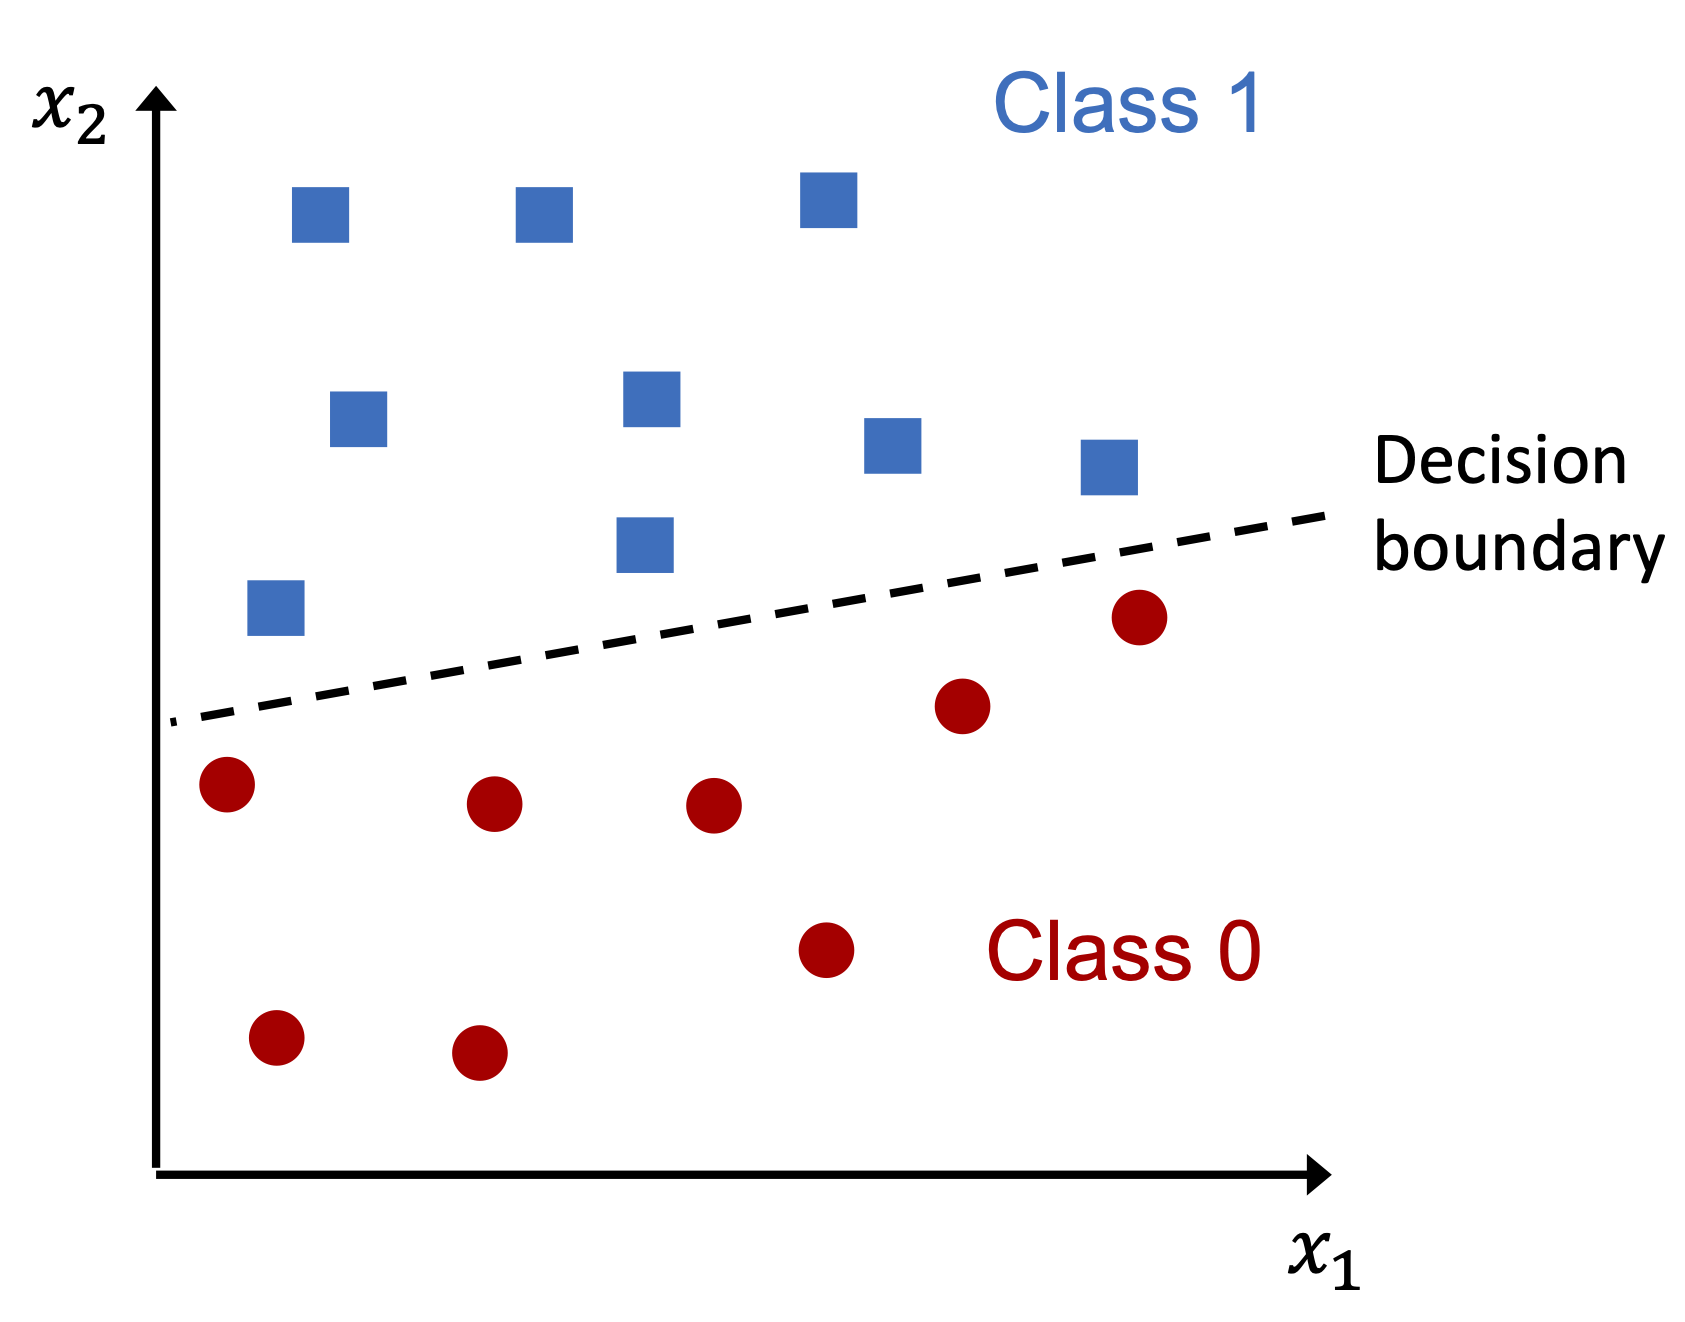
\includegraphics[width=0.4\textwidth]{figures/02_02.png}
	\end{center}
	\begin{itemize}
		\item Binary classification task with two classes: 0 and 1
		\item We can construct a linear decision boundary
		\item We use a threshold function for discriminating among the  two classes
		\item The decision function takes as input a linear combination of the features, that is $\mathbf{z = w^{\top}x + b}$ (net input)
	\end{itemize}
\end{frame}

\begin{frame}{ADALINE: ADAptive LInear NEurons}
%	KEY DIFFERENCE: the weights are updated based on a linear activation function rather than a unit step function like in the perceptron: \high{$\sigma(z) = z$ (identity function)}.
	\begin{center}    
		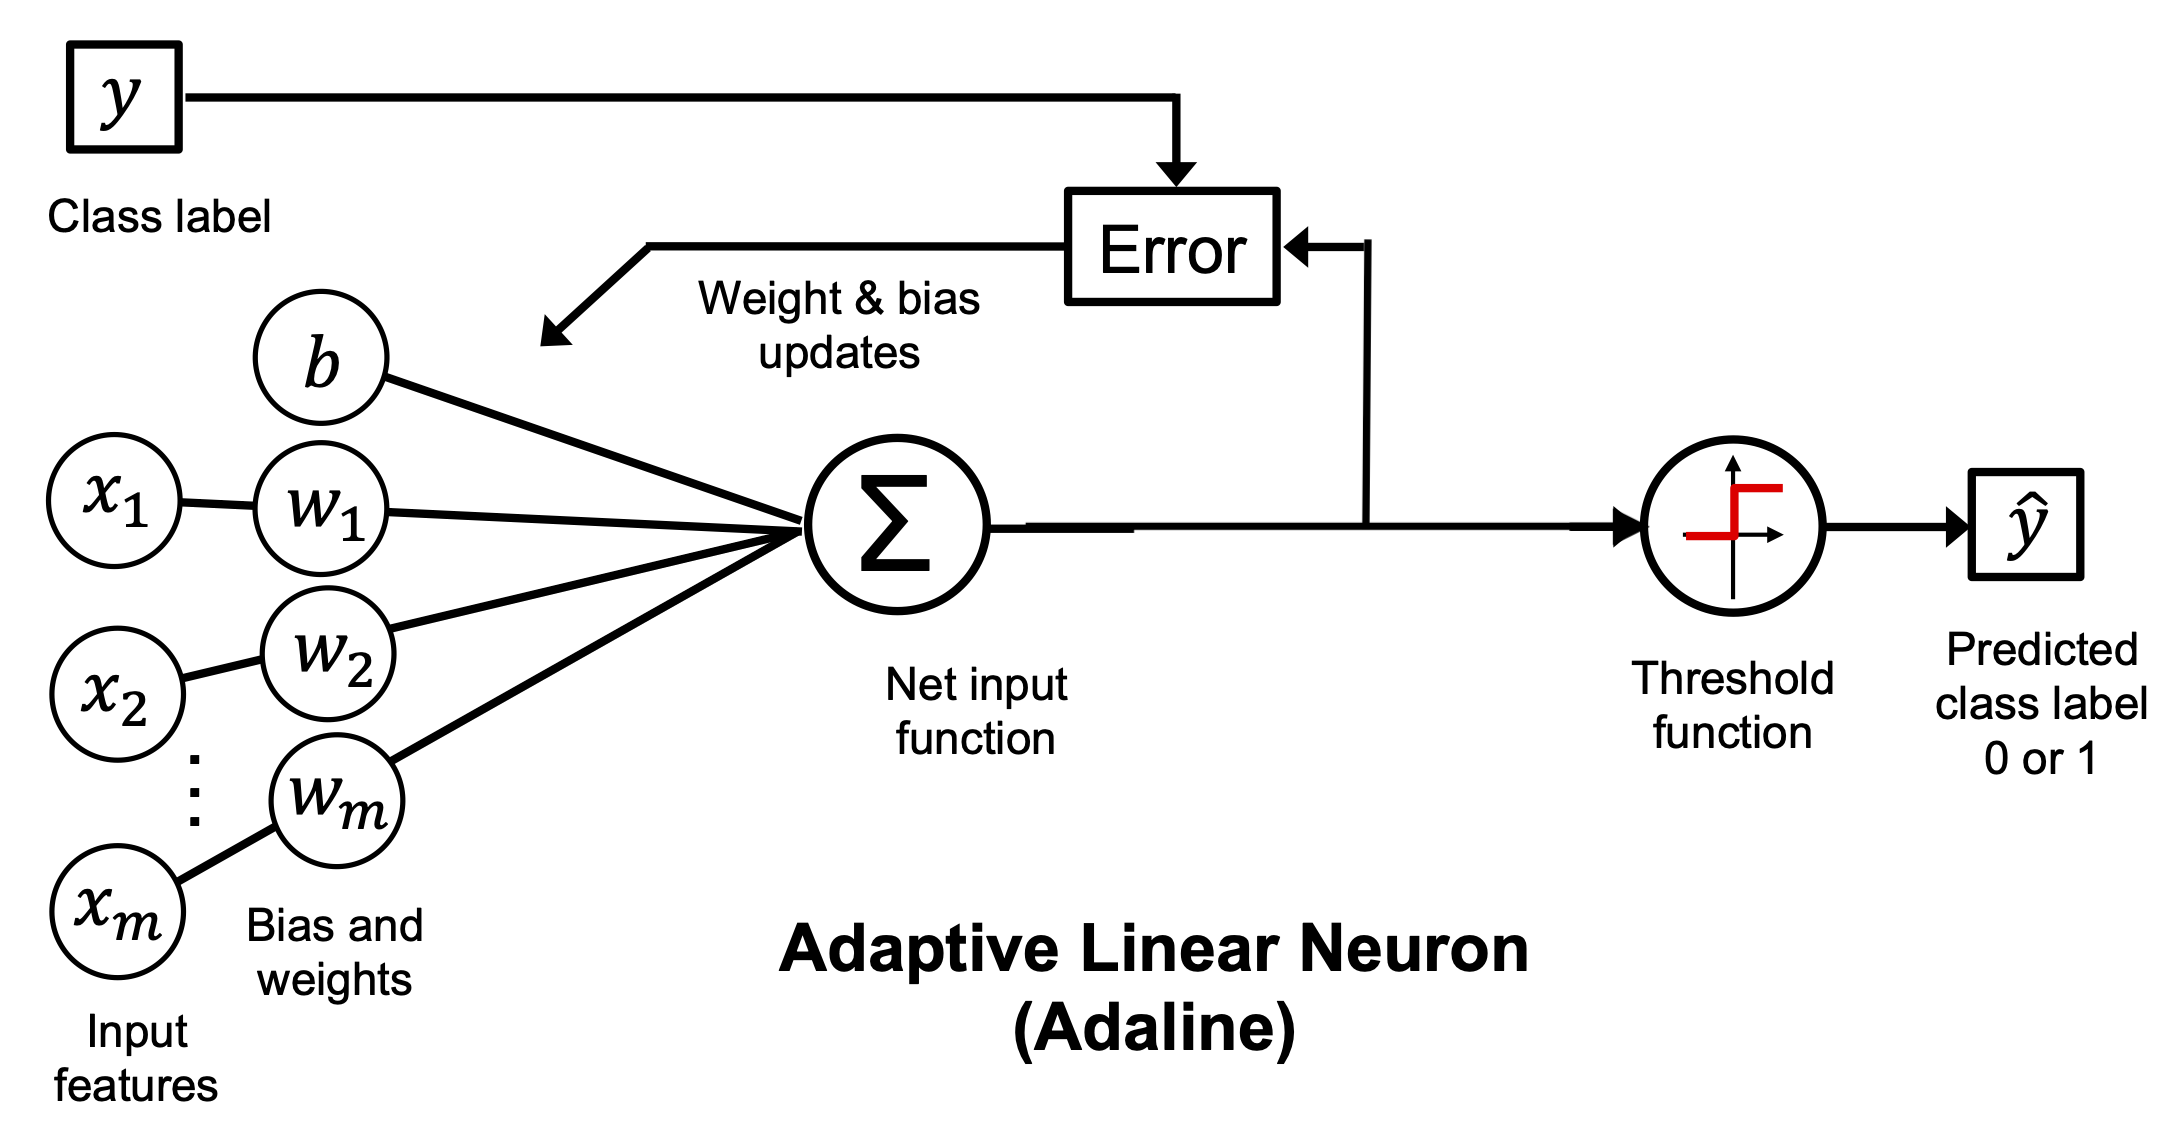
\includegraphics[width=0.75\textwidth]{figures/02_09_new.png}
	\end{center}
%	NOTICE THAT: while the linear activation function is used for learning the weights, we still use a threshold function to make the final prediction (similarly to the perceptron).
\end{frame}

\begin{frame}{Step 1. Updating the weights}
ADALINE rule
		\begin{enumerate}
			\item We initialize the weights and bias;
			\item We compute the NET INPUT: $z^{(i)} = \mathbf{w}^{\top}x^{(i)} + b$;
			%\item We apply a \high{activation function}: $\sigma(z^{(i)}) = z^{(i)}$;
			\item We compute the error in the training step BY $y^{(i)}- z^{(i)}$, where now $y^{(i)}\in \{0, 1\}$ but $z^{(i)}$ takes values in all $\mathbb{R}$;
		\end{enumerate}	
	
	\vfill
	
	Since we want to minimize the difference $y^{(i)}-z^{(i)}$:
	\begin{itemize}
		\item For those $x^{(i)}$ corresponding to $y^{(i)} = 1$, the weights $\mathbf{w}$ and $b$ needs to \emph{push $z^{(i)}$ as closed as possible to $1$};
		\item  For those $x^{(i)}$ corresponding to $y^{(i)} = 0$, the weights $\mathbf{w}$ and $b$ needs to \emph{push $z^{(i)}$ as closed as possible to $0$}.
	\end{itemize}
\end{frame}

\begin{frame}{Step 2. We use a threshold function to make the final prediction}
	\begin{itemize}
		\item At the end of the training, we get $z^{(i)}$ which will not be $0$ or $1$ as we need!! (we need to identify a class);
		\item The  $\high{z^{(i)}}$ will take some values close to $0$ or $1$;
		\item We need then to "transform" them by applying a threshold function;
%		\item Does the threshold function $\sigma^{\high{t}}$ previously defined work here?
		\uncover<2->{
			\vfill\item A possible threshold function:
			$\hat{y}^{(i)}  = 
			\begin{cases}
				1 & \mbox{ if } z^{(i)} \ge 0.5\\
				0 & \mbox{ if } z^{(i)} < 0.5
			\end{cases}$;
			\vfill\item REMEMBER THAT THE THRESHOLD FUNCTION IS ONLY USED TO MAKE THE FINAL PREDICTION!
		}
	\end{itemize}
\end{frame}

\begin{frame}{The optimization algorithm via gradient descent} 
	\begin{center}    
		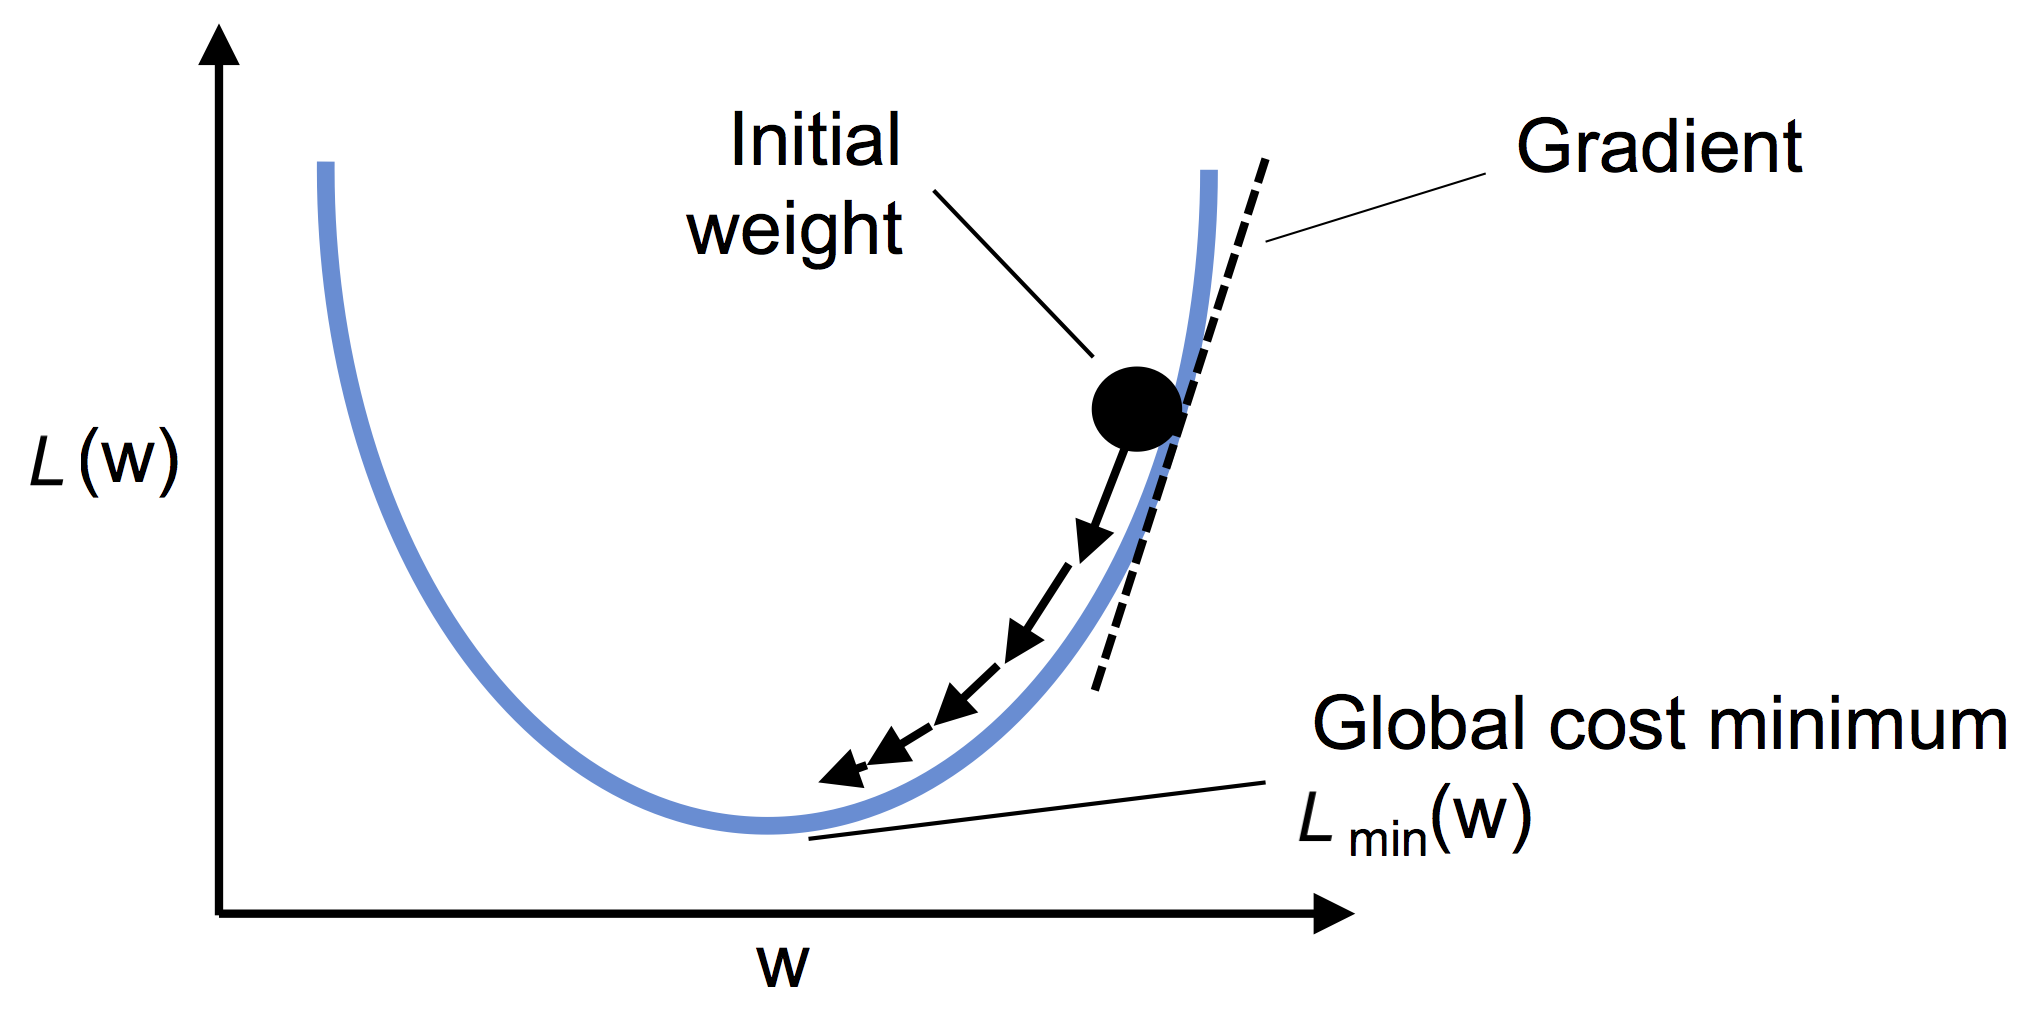
\includegraphics[width=0.4\textwidth]{figures/02_10.png}
	\end{center}
	\begin{itemize}
		\item We use again the  \textbf{mean squared error (MSE)} loss function:
		\begin{equation*}
			%L(\{y^{(i)}\}_{i=1}^n, \{\hat{y}^{(i)}\}_{i=1}^n)
			L(\mathbf{w}, b) =  \frac{1}{2n}\sum_{i=1}^{n}\left(y^{(i)}-z^{(i)}\right)^2
		\end{equation*}
		where now the residuals are computed between the observations and the net inputs
		\item We take a step in the opposite direction of the gradient
		\item The step size is determined by the learning rate and by the slope of the gradient
	\end{itemize}
\end{frame}


\begin{frame}{The rule}
	\begin{itemize}
		\item By gradient descent, we update the model parameters by taking a step in the opposite direction of the gradient of the loss function:
		\begin{align*}
			&\mathbf{w} = \mathbf{w} + \Delta \mathbf{w} &\mbox{with }\Delta \mathbf{w}  = -\eta \nabla_{w}L(\mathbf{w}, b) \\
			&b = b + \Delta b &\mbox{with }\Delta b = -\eta \nabla_{b}L(\mathbf{w}, b)
		\end{align*}
		\item $\nabla_{w}L(\mathbf{w}, b)$ is the vector whose components are the partial derivatives of the loss function with respect to each weight $w_j$:
		\begin{equation*}
			\nabla_{w}L(\mathbf{w}, b) = \begin{pmatrix}
				\frac{\partial L}{\partial w_1} & \frac{\partial L}{\partial w_2}  & \cdots & \frac{\partial L}{\partial w_m} \end{pmatrix}^\top \mbox{ with }
			\frac{\partial L}{\partial w_j} = -\frac{1}{n} \sum_{i=1}^{n}\left(y^{(i)}-z^{(i)}\right) x_j^{(i)};
		\end{equation*}
		\item $\nabla_{b}L(\mathbf{w}, b)$ corresponds to the partial derivative of the loss function with respect to the bias $b$:
		\begin{equation*}
			\nabla_{b}L(\mathbf{w}, b) =  \frac{\partial L}{\partial b} = -\frac{1}{n} \sum_{i=1}^{n}\left(y^{(i)}-z^{(i)}\right).
		\end{equation*}
	\end{itemize}
\end{frame}

\begin{frame}
    \frametitle{Logistic Regression }
    \begin{center}
        {\LARGE Logistic Regression }
    \end{center}
\end{frame}

\begin{frame}{The logistic regression algorithm}
	\begin{center}    
		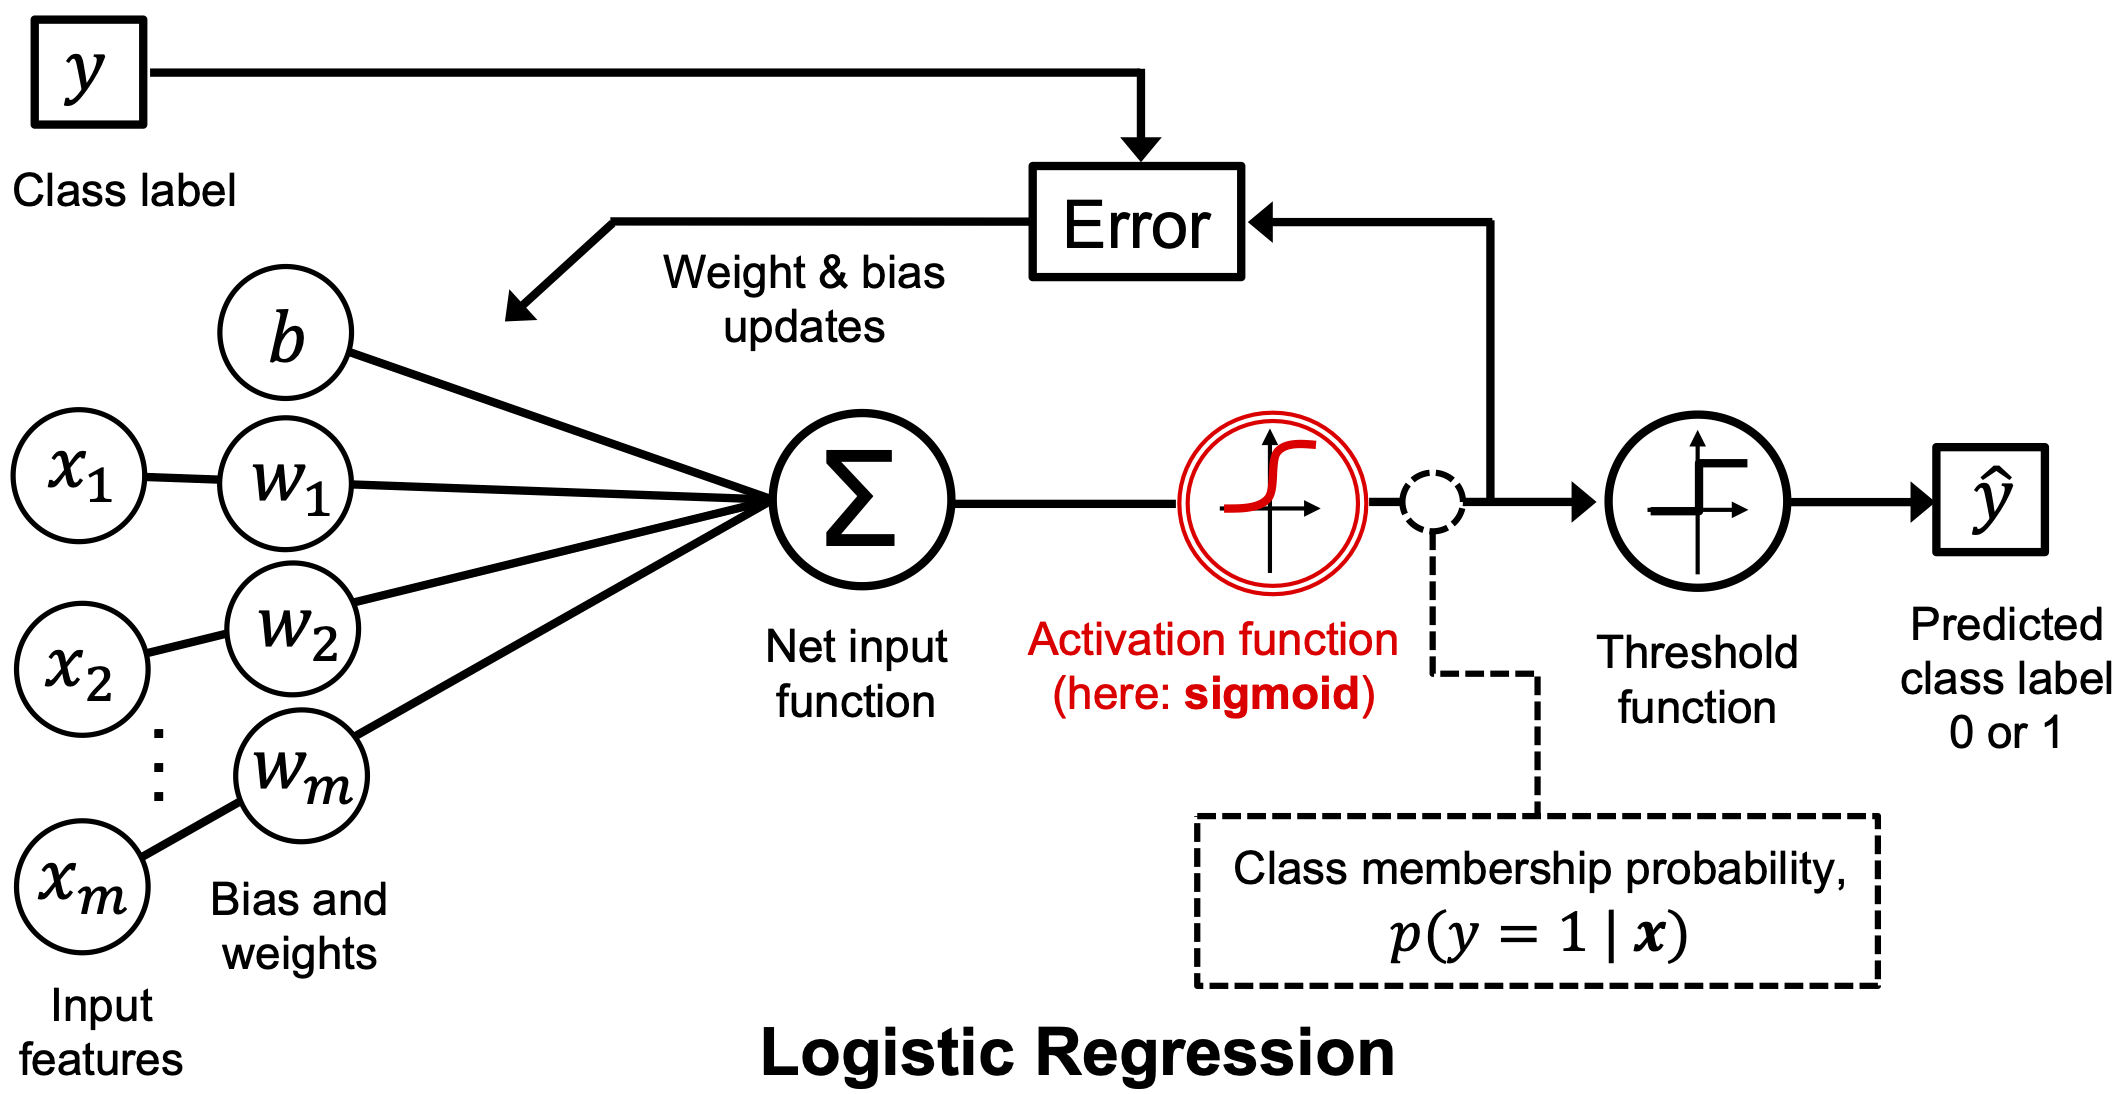
\includegraphics[width=0.8\textwidth]{figures/03_03.png}
	\end{center}
\vfill 
What is this similar to? What is/are the difference(s)?
\end{frame}

\begin{frame}{The sigmoid function}
We define the \textbf{logistic sigmoid function}, or simply \textbf{sigmoid function} by:
	\begin{equation*}
		\sigma(z) := \frac{1}{1+e^{-z}}
	\end{equation*}
where $z =  \mathbf{w}^\top \mathbf{x} + b$ is the net input.

\vfill 


\begin{columns}
	\begin{column}{0.5\textwidth}
			\begin{center}    
			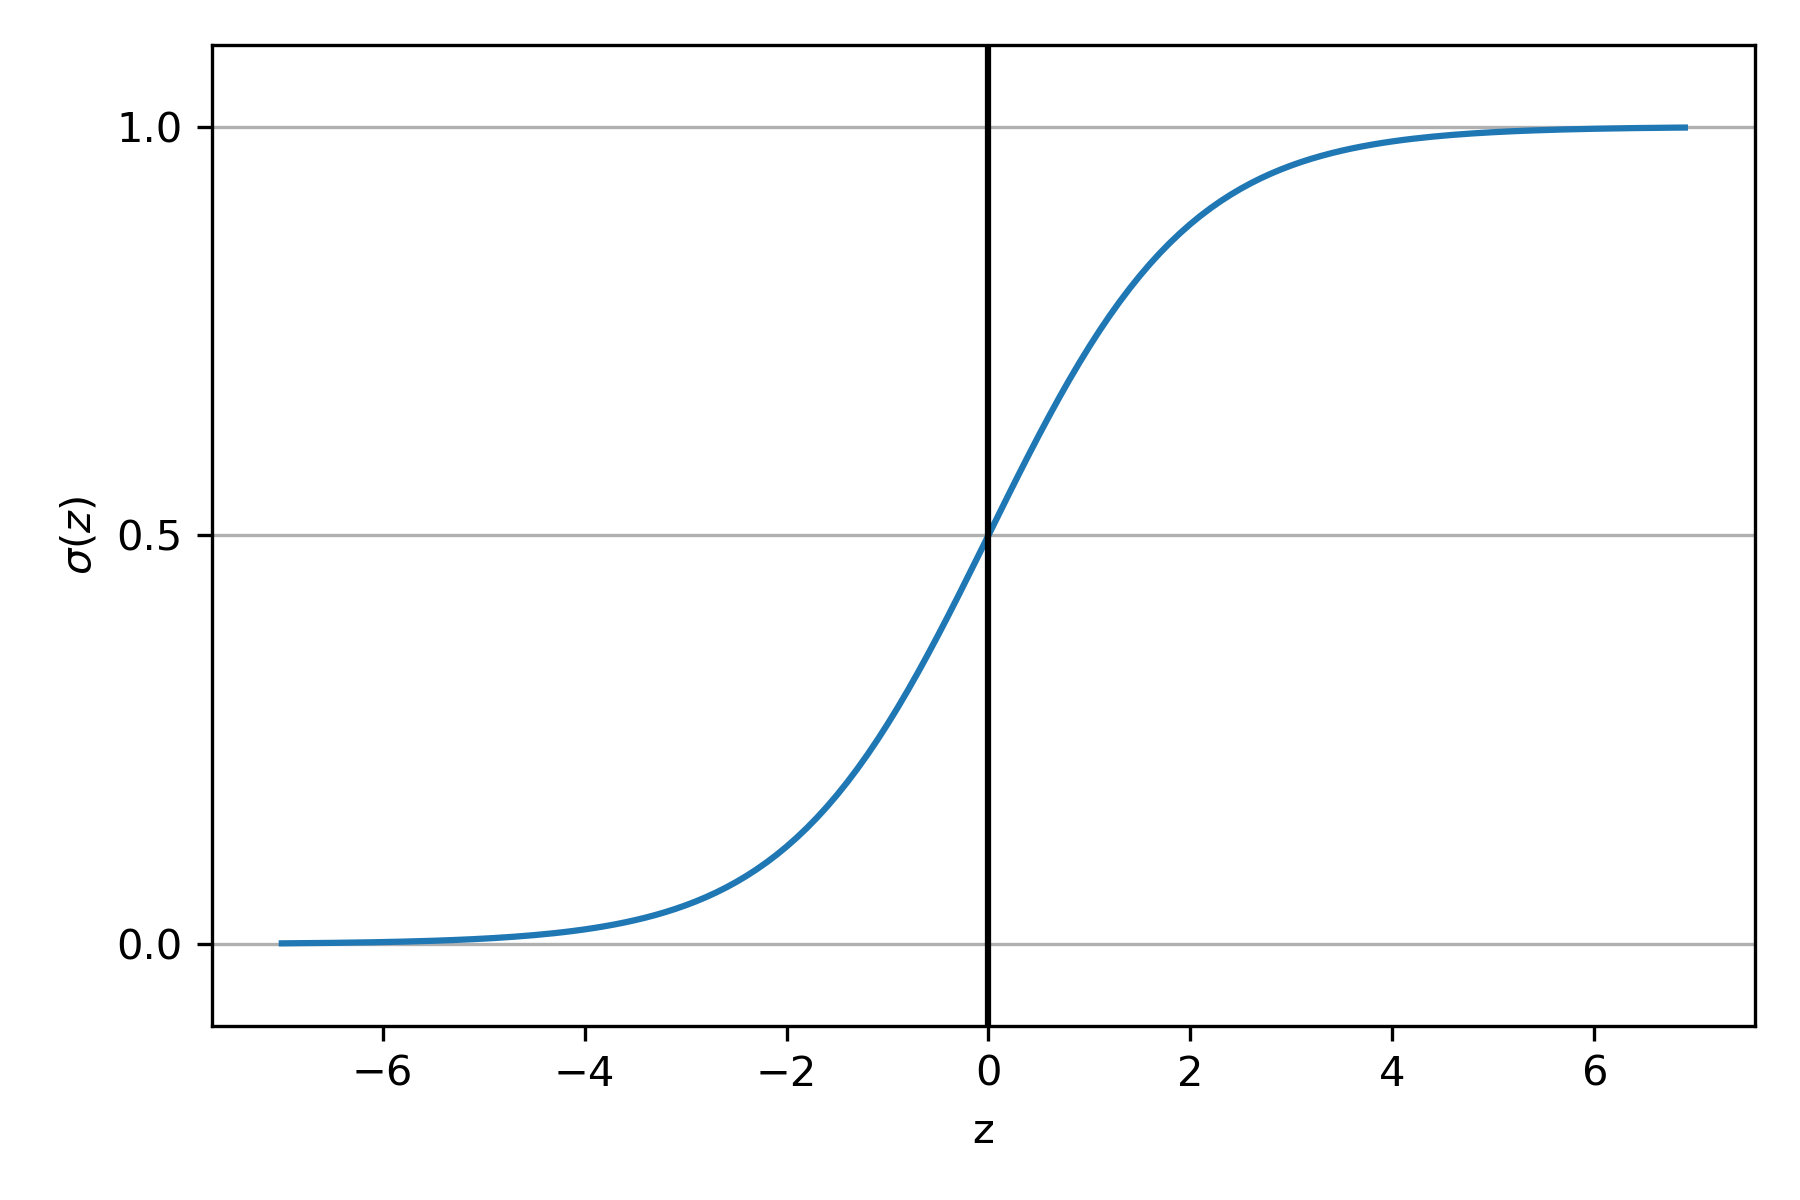
\includegraphics[width=\textwidth]{figures/03_02.png}
		\end{center}
	\end{column}
	\begin{column}{0.5\textwidth}
	Notice that:
	\begin{itemize}
		\item For $z$ approaching $+\infty$, $\sigma(z)$ approaches $1$;
		\item For $z$ approaching $-\infty$, $\sigma(z)$ approaches $0$;
		\item Hence $\sigma: \mathbb{R} \to [0, 1]$ with intercept $\sigma(0) = 0.5$.
	\end{itemize}
\end{column}
\end{columns}
\end{frame}

% \begin{frame}{Why the sigmoid function?}
% %	Before explaining the idea behind the logistic regression, we need the followings:
% %	\begin{itemize}
% Let $p\in [0, 1]$ the probability of a "positive event" (here "positive" does not mean "good", but refers to the event that we want to predict).
% %		\item We define the \textbf{odds} in favor of a particular event as $\frac{p}{1-p}$;
% %		\item We further define the \textbf{logit function}, which is simply the logarithm of the odds:
% %		\begin{equation*}
% %			\mathrm{logit}(p) = \log \frac{p}{1-p},
% %		\end{equation*}
% %		where $\log$ denotes the natural logarithm. Notice that: $\mathrm{logit}: [0, 1]\to \mathbb{R}$.
% %	\end{itemize}
	
% 	\vfill 
	
% 	\begin{block}{Example}
% 		\emph{\small We consider $p$ as the probability that a patient has a certain disease given certain symptoms. Then we think of the positive event as class label $y=1$ and the symptoms as feature $\mathbf{x}$, and \high{$p:= p(y=1|\mathbf{x})$} is the probability that a particular example belongs to the class $1$ given $\mathbf{x}$.}
% 	\end{block}

% 	\vfill 
	
% 	\textbf{The output of the sigmoid function is interpreted as the probability of a particular example belonging to class $1$}:
% 	\begin{equation*}
% 		\high{\sigma(z) = p(y=1|\mathbf{x}; \mathbf{w}, b)}
% 	\end{equation*}
% 	given its features $\mathbf{x}$ and parameterized by the weights and bias,  $\mathbf{w}$ and  $b$. 
	
% 		\begin{block}{Example}
% 			\emph{\small 
% 		If $\sigma(z) = 0.8$ for a particular flower example, it means that the chance that this example is an Iris-versicolor flower is $80\%$.Therefore, the probability that this flower is an Iris-setosa flower can be calculated as $p(y=0|\mathbf{x}; \mathbf{w}, b) = 1- p(y=1|\mathbf{x}; \mathbf{w}, b) = 0.2$, or $20\%$.}
% 	\end{block}

% \end{frame}


\begin{frame}{The (same) threshold function (as Adaline)}
The predicted probability can then simply be converted into a binary outcome via a threshold function:
\begin{equation*}
\hat{y}=	\begin{cases}
		1 & \mbox{if } \sigma(z) \ge 0.5\\
		0 & \mbox{if } \sigma(z) < 0.5
	\end{cases}
\end{equation*}

\begin{block}{Remark}
	\textbf{There are many applications where we are interested in} both the predicted class labels and in \textbf{the estimation of the class-membership probability} (the output of the sigmoid function prior to applying the threshold function). 
\end{block}
Examples:
\begin{itemize}
	\item Weather forecasting: we are interested not only to predict whether it will rain on a particular day, but also to report the chance of rain. 
	\item Medicine: logistic regression can be used to predict the chance that a patient has a particular disease given certain symptoms.
\end{itemize}
\end{frame}

\begin{frame}{What about the learning process?}
	\begin{itemize}
		\item We need to define an objective function that we seek to minimize;
		\item The idea is that we want to \textbf{maximize the likelihood}, namely the probability of classifying the dataset correctly, given some parameters $\mathbf{w}$ and  $b$;
		\item This is equivalent to minimize the \textbf{CROSS-ENTROPY loss function}:
		\begin{equation*}
			\high{L(\mathbf{w}, b) := \sum_{i=1}^{n} \left[  -y^{(i)}\log\left(\sigma(z^{(i)})\right) - (1-y^{(i)})\log\left(1-\sigma(z^{(i)})\right)\right]}.
		\end{equation*}
	\end{itemize}

Example: $n=1$
	\begin{equation*}
		L(\mathbf{w}, b) = -y^{(1)}\log\left(\sigma(z^{(1)})\right) - (1-y^{(1)})\log\left(1-\sigma(z^{(1)})\right)
	\end{equation*}
We notice that:
\begin{equation*}
	L(\mathbf{w}, b)  = \begin{cases}
		-\log\left(\sigma(z^{(1)})\right) & \mbox{if } y^{(1)} = 1\\
		-\log\left(1-\sigma(z^{(1)})\right)& \mbox{if } y^{(1)} = 0
	\end{cases}.
\end{equation*}
	
\end{frame}


\begin{frame}{The cross-entropy function explained}
\begin{columns}
	\begin{column}{0.5\textwidth}
		\begin{equation*}
			L(\mathbf{w}, b)  = \begin{cases}
				-\log\left(\sigma(z^{(1)})\right) & \mbox{if } y^{(1)} = 1\\
				-\log\left(1-\sigma(z^{(1)})\right)& \mbox{if } y^{(1)} = 0
			\end{cases}
		\end{equation*}
	\end{column}
	\begin{column}{0.5\textwidth}
			\begin{center}    
		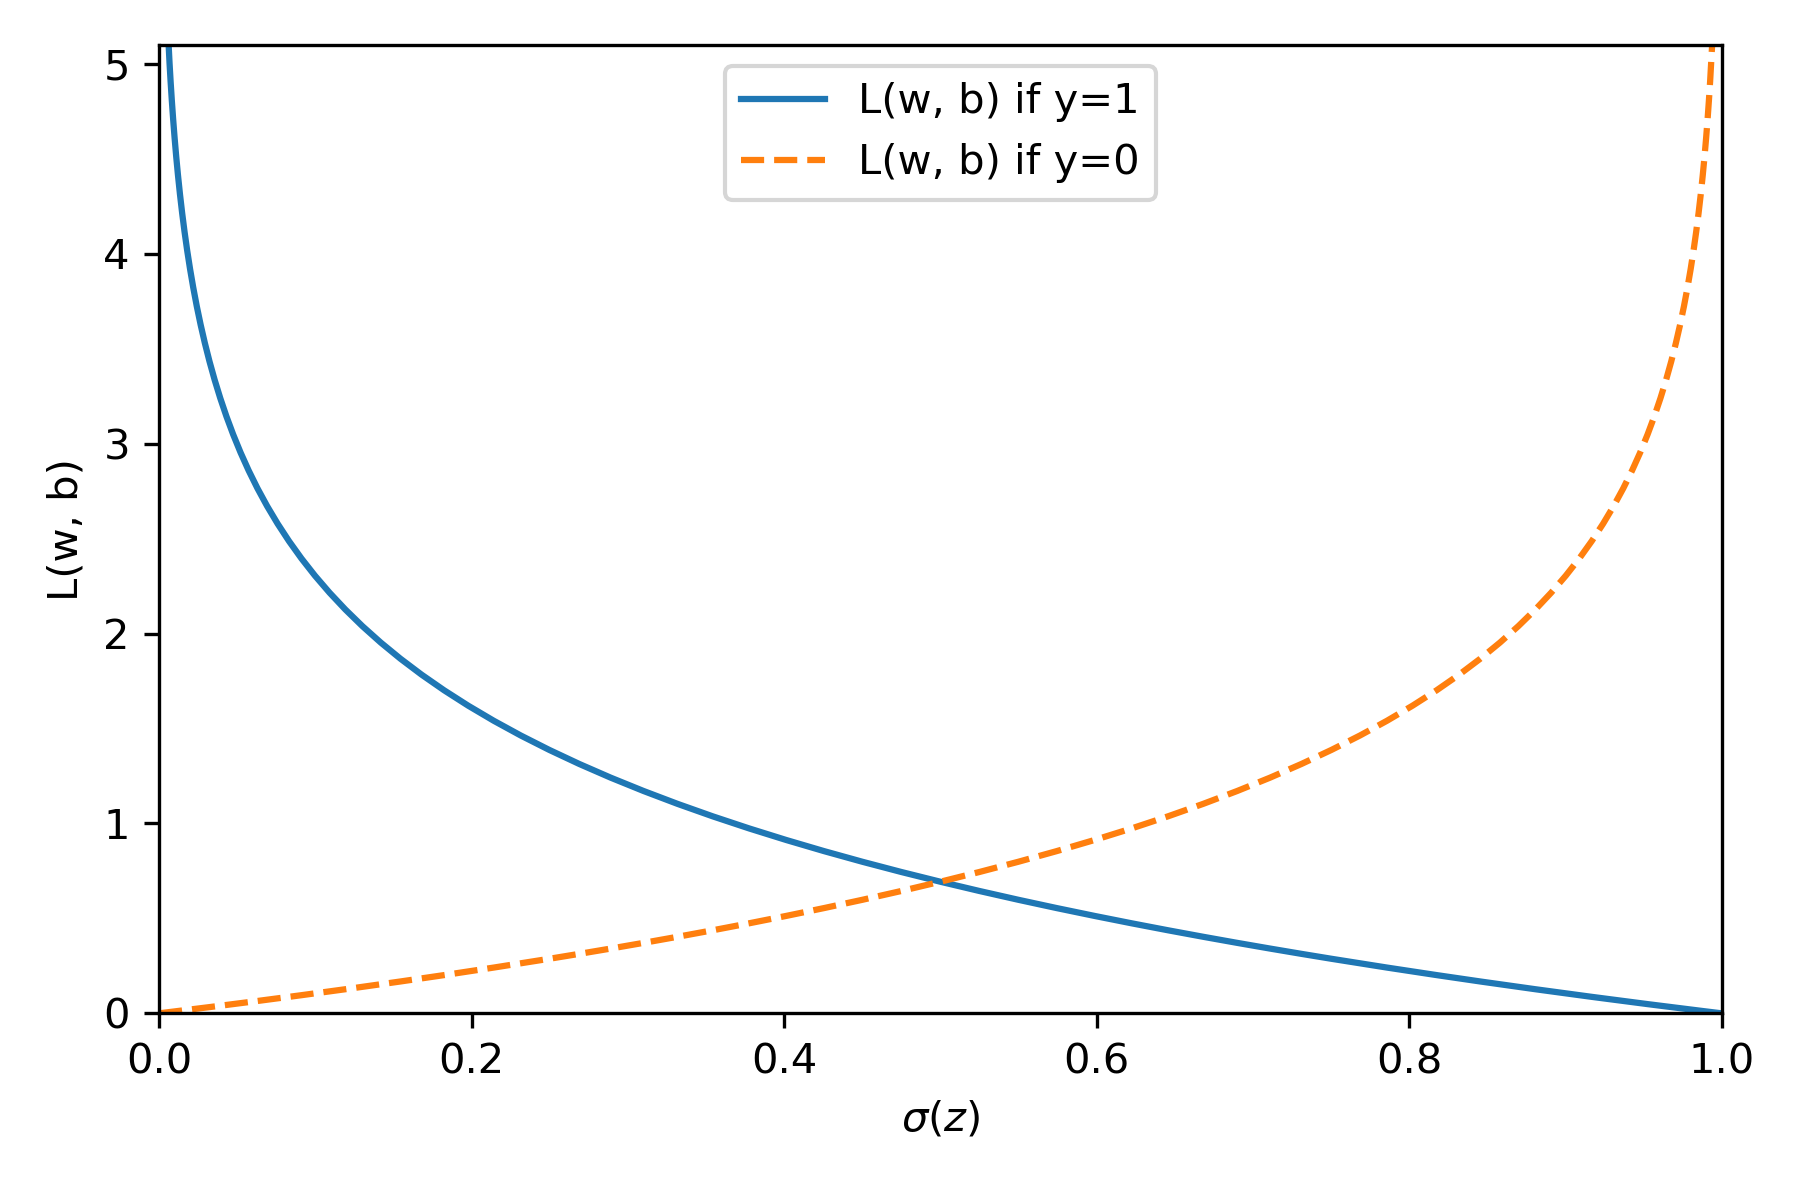
\includegraphics[width=\textwidth]{figures/03_04.png}
	\end{center}
\end{column}
\end{columns}
\begin{itemize}
	\item Blue continuous  line: the loss approaches 0 if we correctly predict that an example belongs to class 1
	\item Orange dashed line: the loss also approaches 0 if we correctly predict $y = 0$
	\item If the prediction is wrong, the loss goes toward infinity
	\item \textbf{We penalize wrong predictions with an increasingly larger loss!}
\end{itemize}
\end{frame}


\begin{frame}{The algorithm}
The logistic regression algorithm can be obtained starting from the Adaline implementation:
\begin{enumerate}
	\item By substituting the MSE loss function with the cross-entropy loss function
	\item By changing the linear activation function with the sigmoid function
\end{enumerate}

\vfill 

\begin{itemize}
	\item What about the gradient for the optimization step?
	\uncover<2->{\item  Using calculus, we can show (optional exercise at home) that \textbf{the parameter updates via gradient descent are equal to the ones for Adaline}, namely the gradient step is unchanged!}
\end{itemize}
\end{frame}

\begin{frame}{The gradient step (unchanged)}
	\begin{itemize}
		\item By \textbf{gradient descent}, we update the model parameters by taking a step in the opposite direction of the gradient of the loss function:
		\begin{align*}
			&\mathbf{w} = \mathbf{w} + \Delta \mathbf{w} &\mbox{with }\Delta \mathbf{w}  = -\eta \nabla_{w}L(\mathbf{w}, b) \\
			&b = b + \Delta b &\mbox{with }\Delta b = -\eta \nabla_{b}L(\mathbf{w}, b)
		\end{align*}
		\item $\nabla_{w}L(\mathbf{w}, b)$ is the vector whose components are the partial derivatives of the loss function with respect to each weight $w_j$:
		\begin{equation*}
			\nabla_{w}L(\mathbf{w}, b) = \begin{pmatrix}
				\frac{\partial L}{\partial w_1} & \frac{\partial L}{\partial w_2}  & \cdots & \frac{\partial L}{\partial w_m} \end{pmatrix}^\top \mbox{ with }
			\high{\frac{\partial L}{\partial w_j} = -\frac{1}{n} \sum_{i=1}^{n}\left(y^{(i)}-\sigma(z^{(i)})\right) x_j^{(i)}};
		\end{equation*}
		\item $\nabla_{b}L(\mathbf{w}, b)$ corresponds to the partial derivative of the loss function with respect to the bias $b$:
		\begin{equation*}
			\nabla_{b}L(\mathbf{w}, b)=   \high{\frac{\partial L}{\partial b} =-\frac{1}{n} \sum_{i=1}^{n}\left(y^{(i)}-\sigma(z^{(i)})\right)}.
		\end{equation*}
	\end{itemize}
\end{frame}



\frame{
    \frametitle{Coding Demo: Building an Automatic Differentiation Engine}
    \begin{itemize}
        \item We will now build a simple automatic differentiation engine from scratch (in code) to illustrate backpropagation in action.
        \item This engine will construct a computational graph during the forward pass and then automatically compute gradients via backprop (chain rule) in the backward pass.
        \item We'll use it to optimize a small example by gradient descent - seeing how the code mirrors the math.
        %This hands-on approach follows Karpathy’s micrograd project, showing that with ~100 lines of code we can implement core backprop functionality!
    \end{itemize}
}




\end{document}